% You should title the file with a .tex extension (hw1.tex, for example)
\documentclass[11pt]{article}

\usepackage{hyperref}
\usepackage{amsmath}
\usepackage{mathtools}
\usepackage{amssymb}
\usepackage{wrapfig}
\usepackage{fancyhdr}
\usepackage{tikz-qtree}
\usepackage{tikz-qtree-compat}
\usepackage[normalem]{ulem}
\usepackage{tikz}
\usepackage{graphicx}
\DeclareMathOperator*{\argmin}{argmin}
\DeclareMathOperator*{\argmax}{argmax}

\oddsidemargin0cm
\topmargin-2cm     %I recommend adding these three lines to increase the 
\textwidth16.5cm   %amount of usable space on the page (and save trees)
\textheight23.5cm  

\newcommand{\question}[2] {\vspace{.25in} \hrule\vspace{0.5em}
\noindent{\bf #1: #2} \vspace{0.5em}
\hrule \vspace{.10in}}
\renewcommand{\part}[1] {\vspace{.10in} {\bf (#1)}}

\newcommand{\myname}{Sean Bittner}
\newcommand{\myandrew}{srb2201@columbia.edu}
\newcommand{\myhwnum}{12}

\setlength{\parindent}{0pt}
\setlength{\parskip}{5pt plus 1pt}
 
\DeclarePairedDelimiter\abs{\lvert}{\rvert}%
 %
\pagestyle{fancyplain}
\rhead{\fancyplain{}{\myname\\ \myandrew}}

\begin{document}

\medskip                        % Skip a "medium" amount of space
                                % (latex determines what medium is)
                                % Also try: \bigskip, \littleskip

\thispagestyle{plain}
\begin{center}                  % Center the following lines
{\Large Inverting nonlinear systems with approximately Bernoulli responses} \\
Sean Bittner \\
April 4, 2019 \\
\end{center}

\section{Introduction}
We want to have approximately Bernoulli responses of the SC network in the various conditions.  Before modeling the full task, we should figure out the appropriate way to invert a nonlinear dynamical system with approx. Bernoulli responses in a single condition.  The key question is how to model this ``emergent property" as a moment constraint.  

\section{SC Model}
There are four total units: two in each hemisphere corresponding to the PRO/CONTRA and ANTI/IPSI populations. \\
\begin{center}
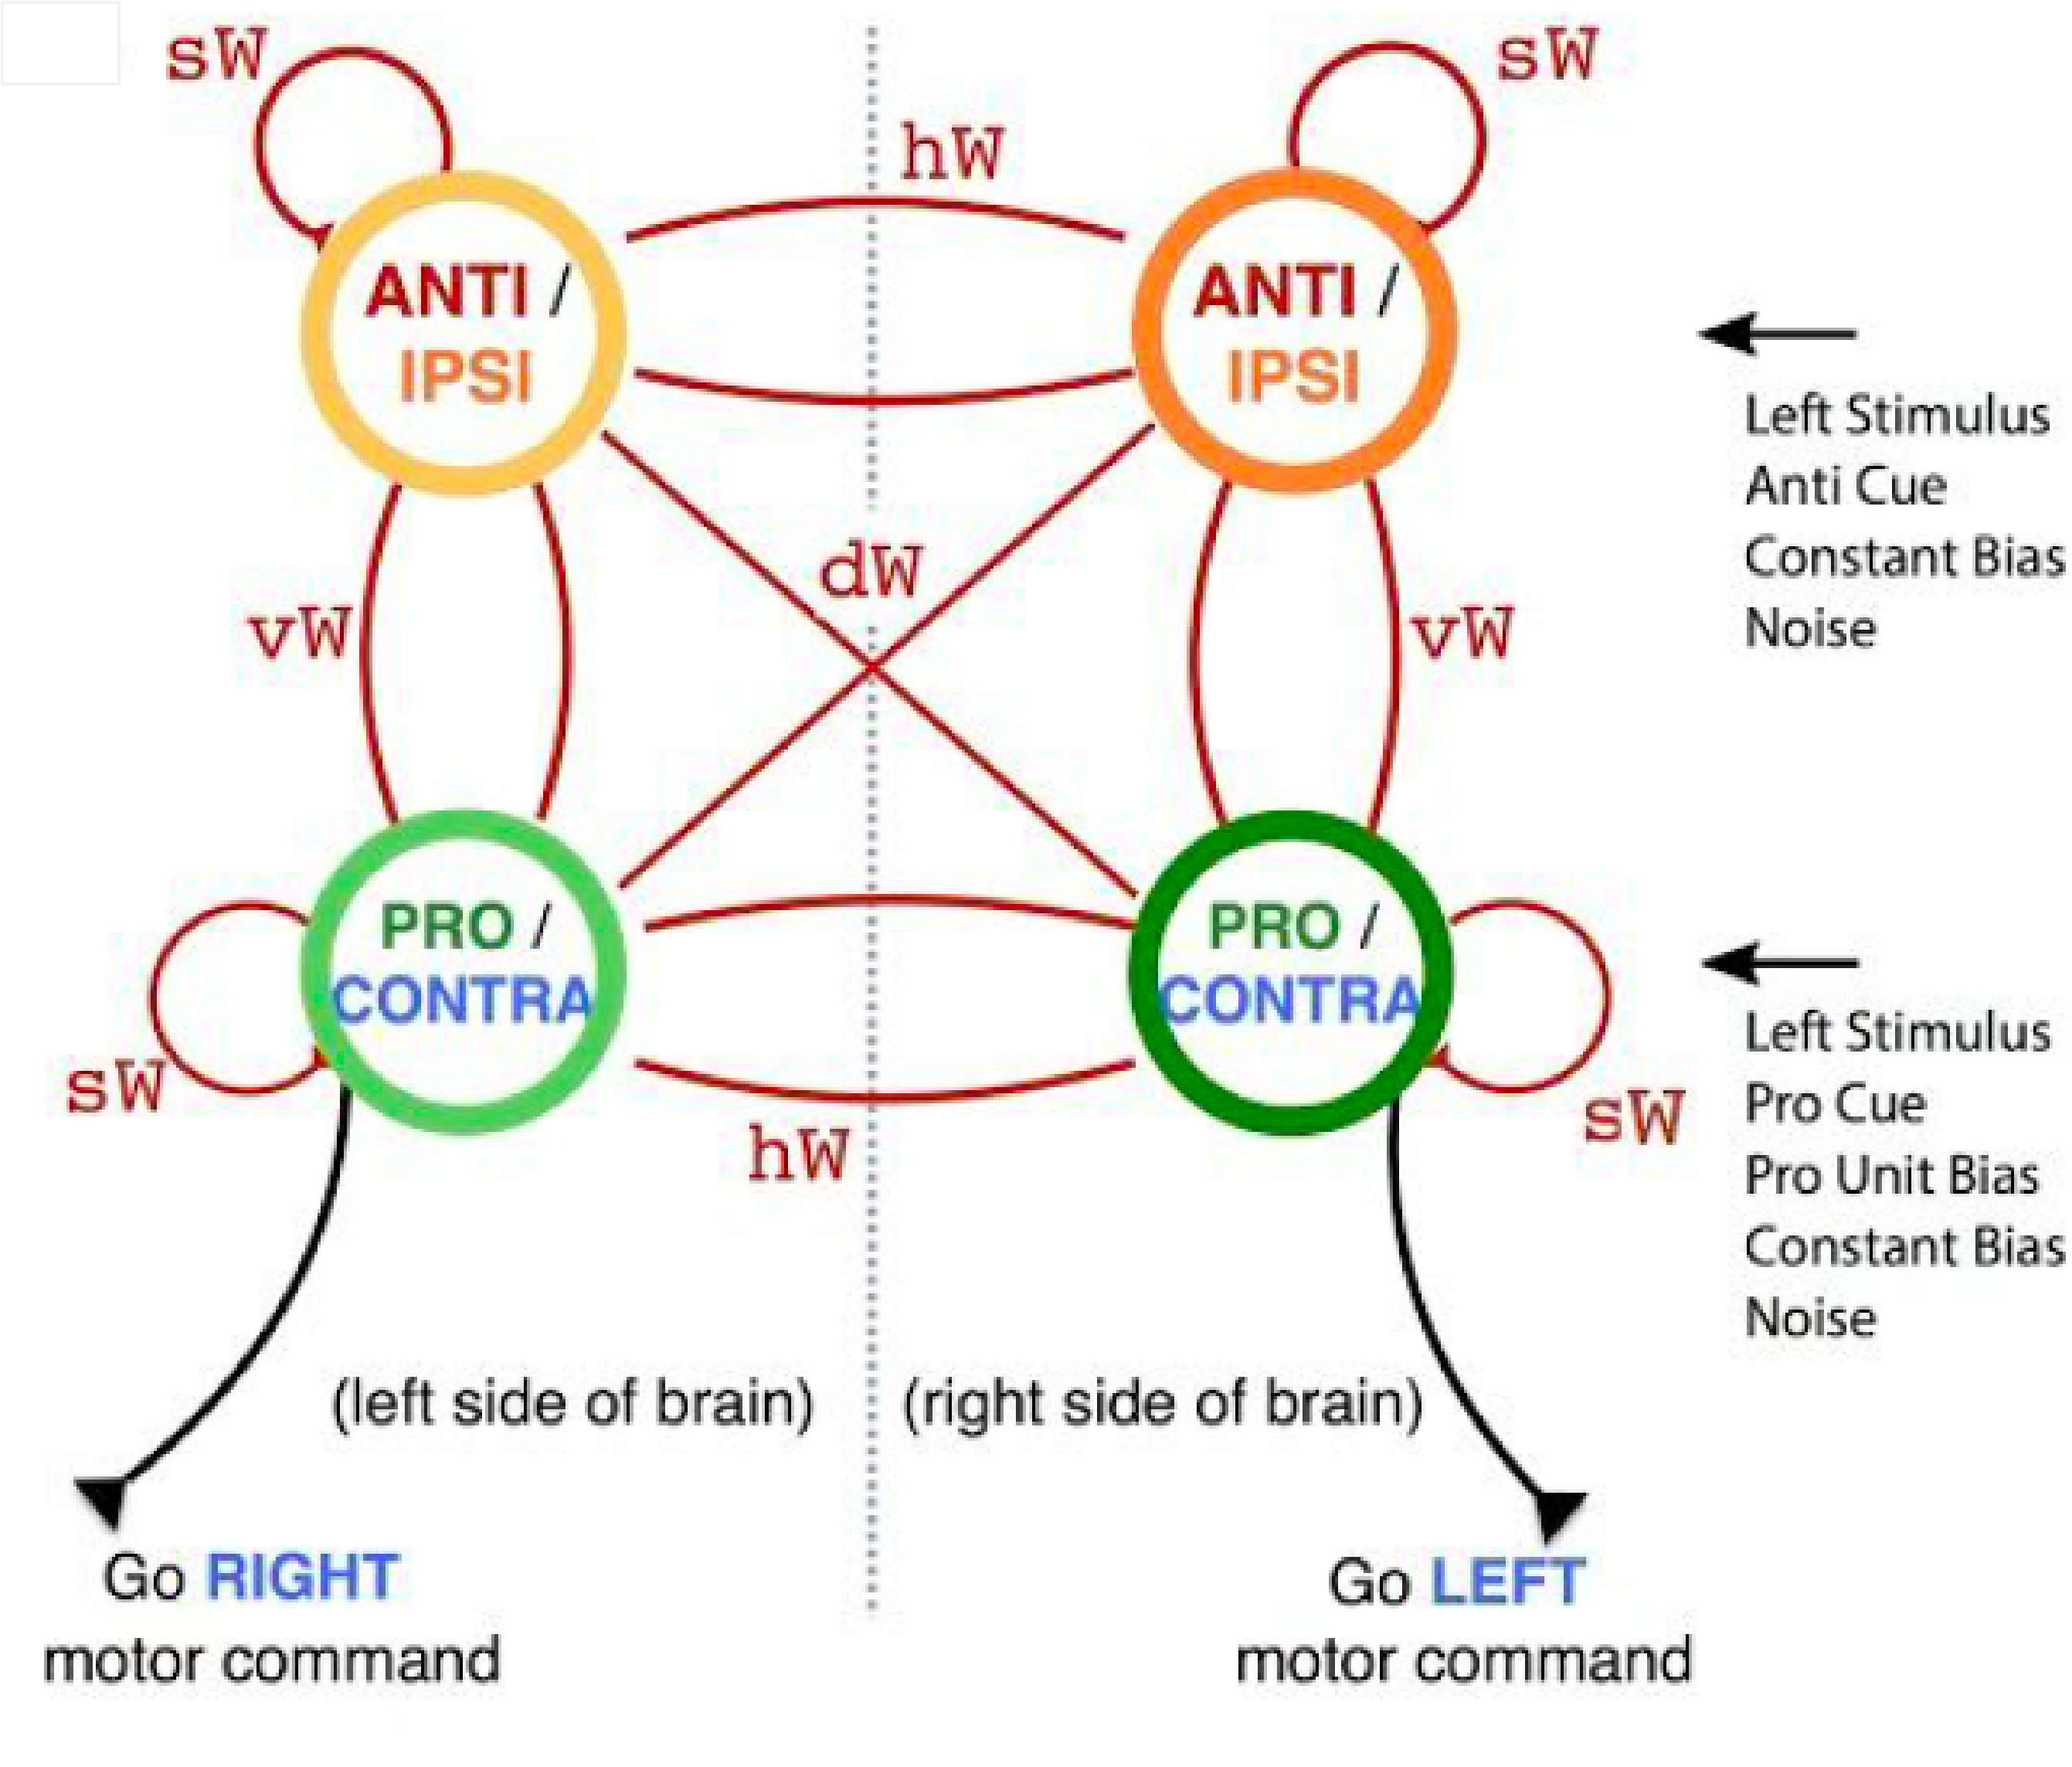
\includegraphics[scale=0.3]{figs/Duan_2019_Fig6_clean.png} 
\end{center}

 Each unit had an external ($V_i$) and internal ($U_i$) variable related by
\begin{equation}
V_i(t) =\eta(t)\left(\frac{1}{2}\tanh\left(\frac{U_i(t) - \theta}{\beta}\right)+ \frac{1}{2} \right)
\end{equation}
$\theta = 0.05$ and $\beta = 0.5$ control the position and shape of the nonlinearity, repsectively, and $\eta(t)$ is the optogenetic inactivation function.

We can order the elements of $V_i$ and $U_i$ into vectors $v$ and $u$ with elements
\begin{equation}
v = \begin{bmatrix} V_{LP} \\ V_{LA} \\ V_{RA} \\ V_{RP} \end{bmatrix} \hspace{2cm} u = \begin{bmatrix} U_{LP} \\ U_{LA} \\ U_{RA} \\ U_{RP} \end{bmatrix}
\end{equation}

 The internal variables follow dynamics:
\begin{equation}
\tau \frac{\partial u}{\partial t} = -u + Wv + I + \sigma \partial W
\end{equation}
with time constant $\tau = 0.09s$ and gaussian noise $\sigma \partial W$ controlled by the magnitude of $\sigma$.  The weight matrix has 8 parameters $sW_P$, $sW_A$, $vW_{PA}$, $vW_{AP}$, $hW_P$, $hW_A$, $dW_{PA}$, and $dW_{AP}$,  related to the depiction in Fig. 2:
\begin{center}
\textbf{Full Model} \\
\end{center}
\begin{equation}
W = \begin{bmatrix} sW_P & vW_{PA} &  dW_{PA} & hW_P \\ vW_{AP}  & sW_A & hW_A  & dW_{AP} \\ dW_{AP} & hW_P & sW_A & vW_{AP}  \\  hW_A & dW_{PA} & vW_{PA}  & sW_P \end{bmatrix}
\end{equation}

The input is a sum of five task-relalated inputs.
\begin{equation}
I = I_{\text{constant}} + I_{\text{pro-bias}} + I_{\text{rule}} + I_{\text{choice-period}} + I_{\text{light}}
\end{equation}

\[I_{\text{constant}}(t) = E_{\text{constant}} \begin{bmatrix} 1 & 1 & 1 & 1 \end{bmatrix}^\top \]
\[I_{\text{P,bias}}(t) = E_{\text{P,bias}} \begin{bmatrix} 1 & 0 & 0 & 1 \end{bmatrix}^\top \]
\[I_{\text{P,rule}}(t) = \begin{cases}
                           E_{\text{P,rule}} \begin{bmatrix} 1 & 0 & 0 & 1 \end{bmatrix}^\top,& \text{if } t\leq 1.2s \\
                            0,              & \text{otherwise}
                         \end{cases}\]
\[I_{\text{A,rule}}(t) = \begin{cases}
                           E_{\text{A,rule}} \begin{bmatrix} 0 & 1 & 1 & 0 \end{bmatrix}^\top,& \text{if } t\leq 1.2s \\
                            0,              & \text{otherwise}
                         \end{cases}\]
\[I_{\text{choice}}(t) = \begin{cases}
                           E_{\text{choice}} \begin{bmatrix} 1 & 1 & 1 & 1 \end{bmatrix}^\top,& \text{if } t > 1.2s \\
                            0,              & \text{otherwise}
                         \end{cases}\]
                         
\[I_{\text{light}}(t) = \begin{cases}
                           E_{\text{light}} \begin{bmatrix} 1 & 1 & 0 & 0 \end{bmatrix}^\top,& \text{if } t > 1.2s \text{and Left} \\
                           E_{\text{light}} \begin{bmatrix} 0 & 0 & 1 & 1 \end{bmatrix}^\top,& \text{if } t > 1.2s \text{and Right} \\
                            0,              & t \leq 1.2s
                         \end{cases}\]
We'll also consider a 4-parameter reduced model:
\begin{center}
\textbf{Reduced Model} \\
\end{center}
\begin{equation}
W = \begin{bmatrix} sW & vW &  dW & hW \\ vW  & sW & hW  & dW \\ dW & hW & sW & vW \\  hW & dW & vW  & sW \end{bmatrix}
\end{equation}

\section{Setting up the DSN behavior constraints}

Let's say that we want to learn the parameters that produce a Bernoulli rate of $p_{LP}$ in the Left, Pro condition.  We'll let $\hat{p}_i$ be the empirical average steady state (ss) response (final $V_{LP}$ at end of task) over M=100 gaussian noise draws for a given dynamical system parameterization $z_i$:

\begin{equation}
 \hat{p}_i = E_{\sigma \partial W} \left[ V_{LP,\text{ss}} \mid s=L, c=P, z_i \right] = \frac{1}{M}\sum_{j=1}^M V_{LP,\text{ss}}(s=L, c=P, z_i, \sigma \partial W_j)
 \end{equation}

The noise is fixed at $\sigma = 0.3$ (the average of satisfactory parameterizations from Duan et al.).  For the 1st constraint, we certainly want the average over DSN samples to be $p_{LP}$:
\begin{equation}
E_{z \sim q_\phi} \left[ E_{\sigma \partial W} \left[ V_{LP,\text{ss}} \mid s=L, c=P, z \right] \right] = E_{z \sim q_\phi} \left[ \hat{p} \right] = p_{LP}
\end{equation}

We can then ask that the variance of the steady state responses across gaussian draws, is the Bernoulli variance for the empirical rate $\hat{p}$.
\begin{equation}
 Var_{\sigma \partial W} \left[ V_{LP,\text{ss}} \mid s=L, c=P, _iz \right] = \hat{p}(1 - \hat{p})
\end{equation}

With DSNs, we enforce constraints in expectation over DSN samples, so we can force Bernoulli responses with this 2nd constraint:
\begin{equation}
E_{z \sim q\phi} \left[ Var_{\sigma \partial W} \left[ V_{LP,\text{ss}} \mid s=L, c=P, _iz \right] - \hat{p}(1 - \hat{p}) \right] = 0
\end{equation}

Since the maximum variance of a random variable bounded from 0 to 1 is the Bernoulli variance ($\hat{p}(1-\hat{p})$), in principal, we do not need to control the second moment (over DSN samples) of this test-static (the variance over gaussian draws).  In reality, these variables are dynamical system states and can only exponentially decay (or saturate) to 0 (or 1), so the Bernoulli variance constraint can only be undershot.  This is important to be mindful of, when thinking about how to enforce Bernoulli responses in this fashion.

\section{Attempt 1: Two constraints}
To begin, I wanted to see if I could train a DSN on the reduced parameterization of the DSN model (4 parameter connectivity matrix) to produce a Bernoulli rate of 0.5.  In Duan et al. 2019, many other parameters are treated as free parameters: \\
\begin{itemize}
\item 8 connectivity params
\item 6 input params -- ($E_{\text{constant}}$, $E_{P,\text{bias}}$, $E_{P,\text{rule}}$, $E_{A,\text{rule}}$, $E_{\text{choice}}$, $E_{\text{light}}$)
\item 1 noise param -- $\sigma$
\item 1 opto param (we're not worried about this yet)
\end{itemize}
For this analysis, I set $E_{\text{constant}} = 0.0$, $E_{P,\text{bias}} = 0.1$, $E_{P,\text{rule}} = 0.5$, $E_{\text{choice}} = -0.2$, $E_{\text{light}} = 0.1$, and $\sigma = 0.3$ as they were the means of Figure S6 in Duan et. al. 2019.  Just because these are the means of the marginalized distribution of satisfactory parameters, does \textbf{not} mean that the joint distribution has samples here. That's something to be mindful of, considering we may be working in a region of parameter space with no satisfactory weight matrices.

 $E_{A,\text{rule}}$ is irrelevant for the LP condition, so it was set to zero.
 
I trained a DSN with batchsize (M=1000) on the reduced (4 weight param) SC model to produce the following behavior:
\[E_{z \sim q_\phi} \left[ \hat{p} \right] = 0.5\]
\[E_{z \sim q\phi} \left[ Var_{\sigma \partial W} \left[ V_{LP,\text{ss}} \mid s=L, c=P, _iz \right] - \hat{p}(1 - \hat{p}) \right] = 0\]

This was with an initialization of augmented lagrangian (AL) parameter $c_0 = 10^{15}$.  All $c$ initializations with exponent 20 or greater had numerical instabilities.  Each of the 5 randomly initialized optimizations of 10 planar flows ran for 40 AL epochs.

\begin{center}
\textbf{Reduced model, p=0.5} \\
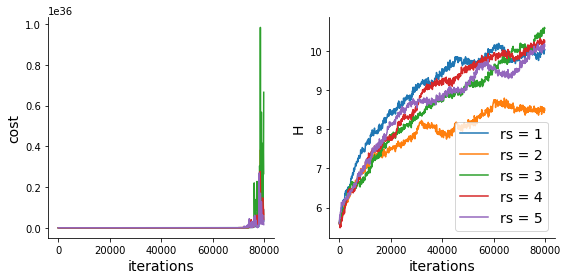
\includegraphics[scale=0.6]{figs/cost_H_SC_reduced_c=15_p=50.png} \\
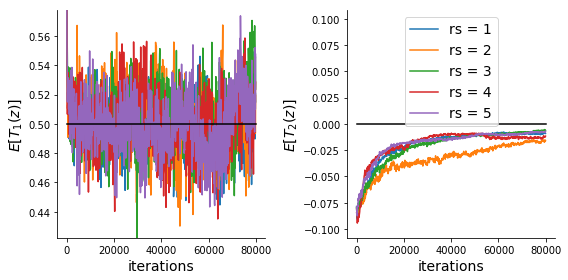
\includegraphics[scale=0.6]{figs/constraints_SC_reduced_c=15_p=50.png}
\end{center}

The rate of 0.5 is matched (bottom left), yet the Bernoulli variance constraint is undershot (bottom right).  Again, there will always be some degree of empirical undershoot for such a constraint.  Notably, after the constraint satisfaction has saturated, the entropy continues to increase substantially.  An important question is whether this increase in entropy is solely driven by the entropy term in the optimization (which is weighted very little) or actually by the choice of constraints.

I ran the same optimization with $c_0 = 0$, dropping the entropy term from the cost function entirely.  Again, we saw constraint adherance saturate, while entropy grows.


\begin{center}
\textbf{Reduced model, no entropy term, p=0.5} \\
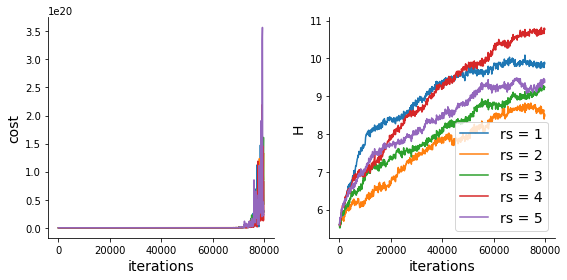
\includegraphics[scale=0.6]{figs/cost_H_SC_reduced_c=0_p=50.png} \\
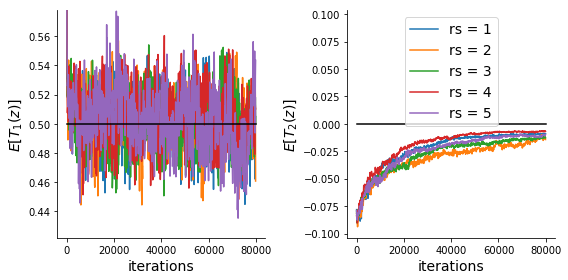
\includegraphics[scale=0.6]{figs/constraints_SC_reduced_c=0_p=50.png}
\end{center}

To understand why entropy is growing, it may be insightful to look at the distributions underlying the mean sufficient statistics of the behavior.  Below, I've plotted the $\hat{p}$ and Bernoulli variance error across DSN samples at the end of optimization for each initialization.
\begin{center}
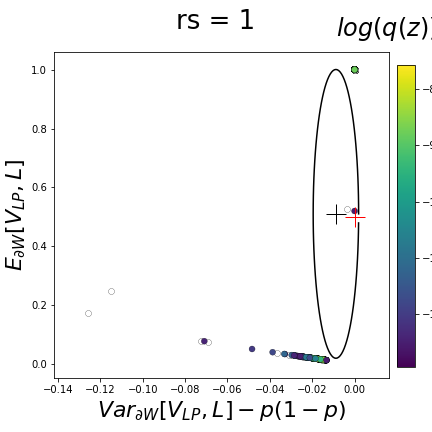
\includegraphics[scale=0.33]{figs/T_x_SC_reduced_c=0_p=50_rs=1.png}
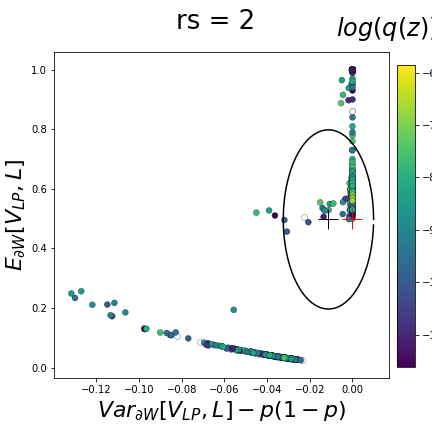
\includegraphics[scale=0.33]{figs/T_x_SC_reduced_c=0_p=50_rs=2.png}
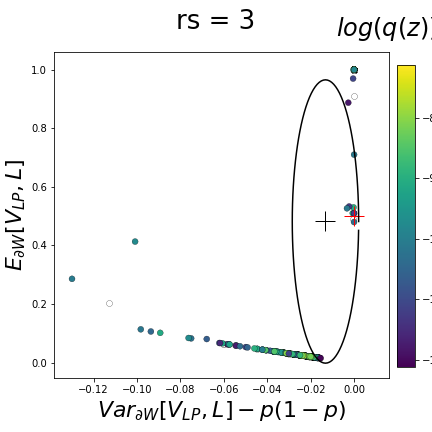
\includegraphics[scale=0.33]{figs/T_x_SC_reduced_c=0_p=50_rs=3.png} \\
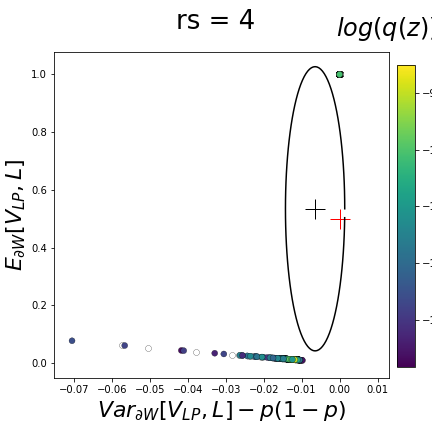
\includegraphics[scale=0.33]{figs/T_x_SC_reduced_c=0_p=50_rs=4.png}
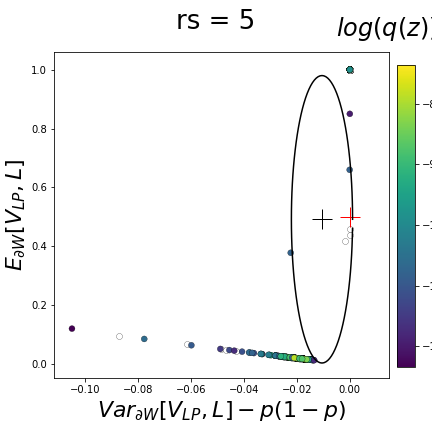
\includegraphics[scale=0.33]{figs/T_x_SC_reduced_c=0_p=50_rs=5.png}
\end{center}

The DSN is producing a bimodal distribution of networks that grow to saturation in $V_{LP}$, and half that decay to zero every time (no variance).  This is makes sense in the DSN parameter distributions which have a connectivity mode in each of the all-positive and all-negative ``quartants." 

\begin{center}
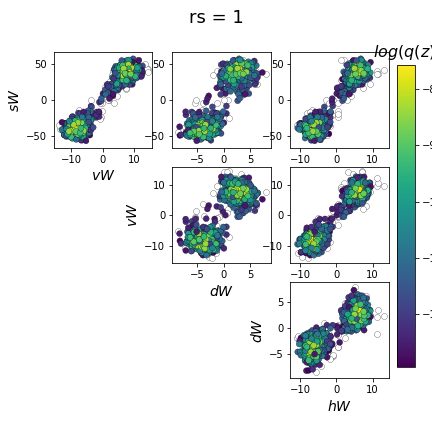
\includegraphics[scale=0.33]{figs/Z_SC_reduced_c=0_p=50_rs=1.png}
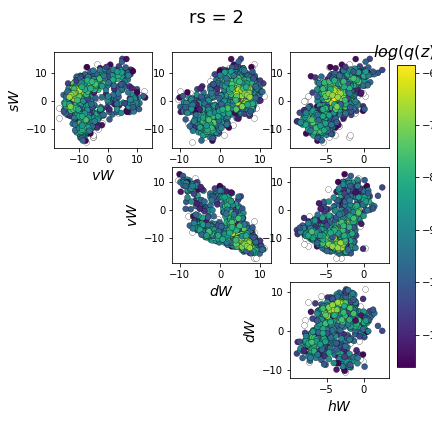
\includegraphics[scale=0.33]{figs/Z_SC_reduced_c=0_p=50_rs=2.png}
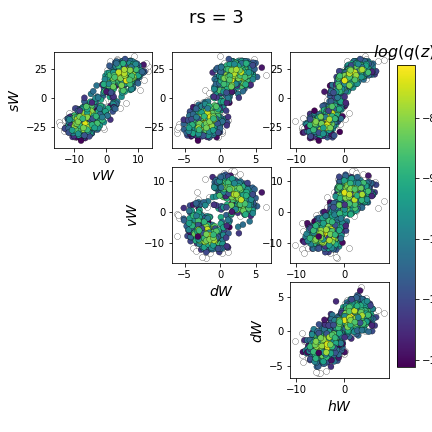
\includegraphics[scale=0.33]{figs/Z_SC_reduced_c=0_p=50_rs=3.png} \\
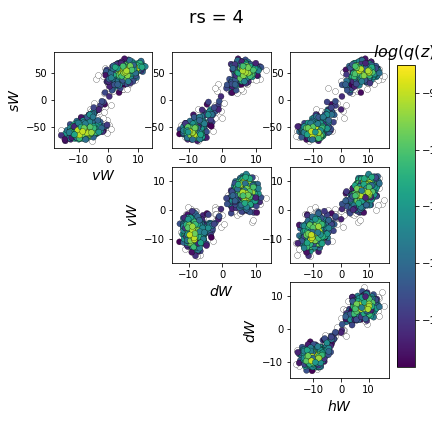
\includegraphics[scale=0.33]{figs/Z_SC_reduced_c=0_p=50_rs=4.png}
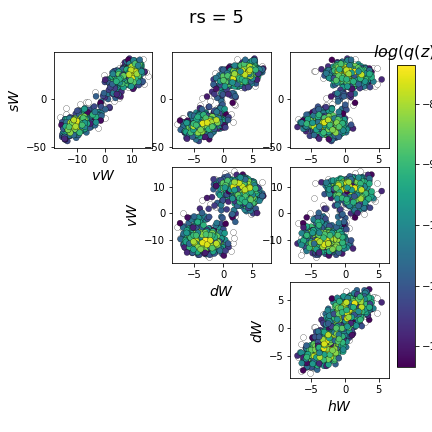
\includegraphics[scale=0.33]{figs/Z_SC_reduced_c=0_p=50_rs=5.png}
\end{center}

I wondered if the full mode (8-param connectivity) would fair better in constraint satisfaction, but that did not happen.

\begin{center}
\textbf{Full model, no entropy term, p=0.5} \\
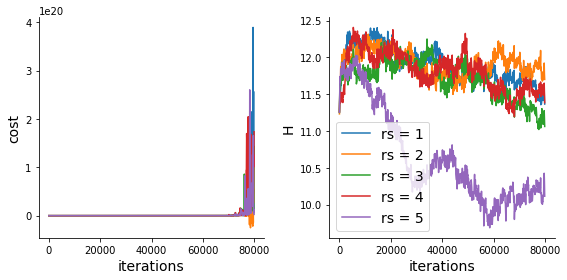
\includegraphics[scale=0.6]{figs/cost_H_SC_full_c=0_p=50.png} \\
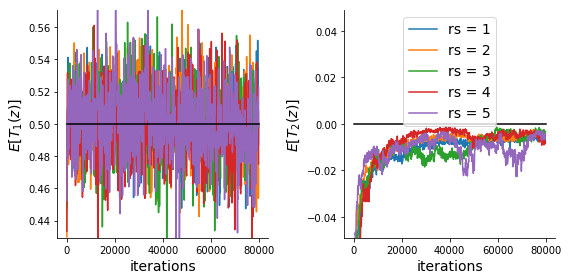
\includegraphics[scale=0.6]{figs/constraints_SC_full_c=0_p=50.png}
\end{center}
\begin{center}
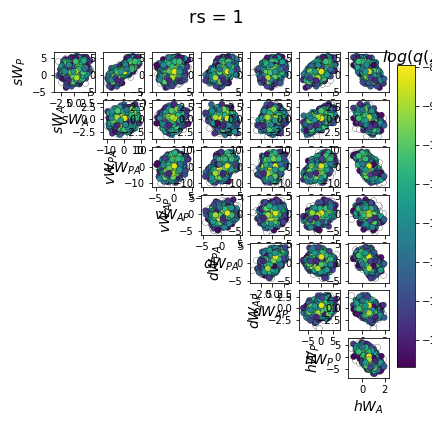
\includegraphics[scale=0.33]{figs/Z_SC_full_c=0_p=50_rs=1.png}
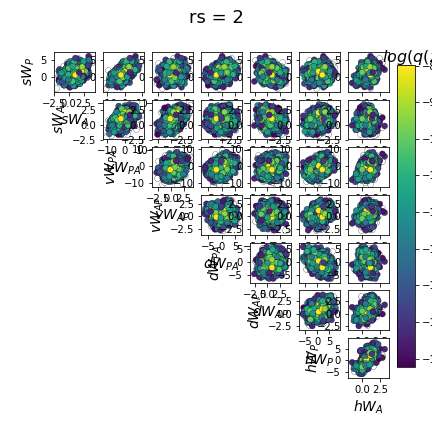
\includegraphics[scale=0.33]{figs/Z_SC_full_c=0_p=50_rs=2.png}
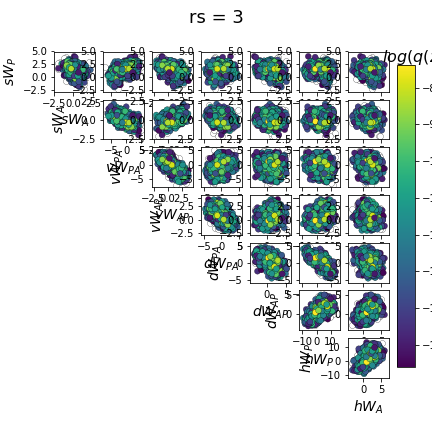
\includegraphics[scale=0.33]{figs/Z_SC_full_c=0_p=50_rs=3.png} \\
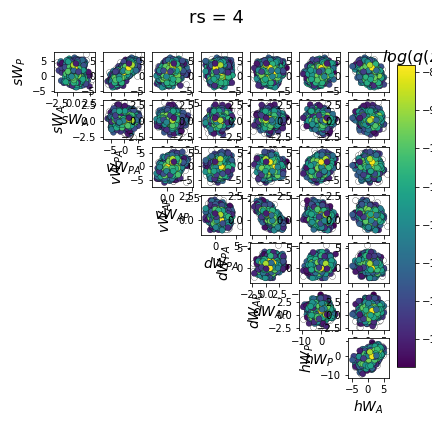
\includegraphics[scale=0.33]{figs/Z_SC_full_c=0_p=50_rs=4.png}
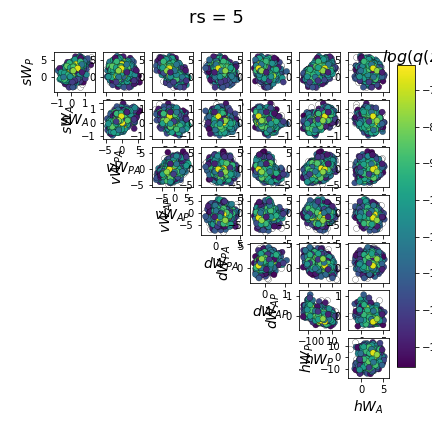
\includegraphics[scale=0.33]{figs/Z_SC_full_c=0_p=50_rs=5.png}
\end{center}
\begin{center}
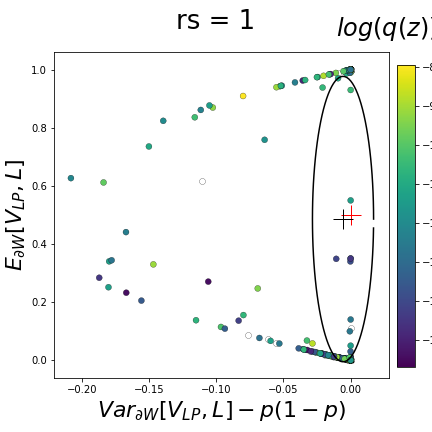
\includegraphics[scale=0.33]{figs/T_x_SC_full_c=0_p=50_rs=1.png}
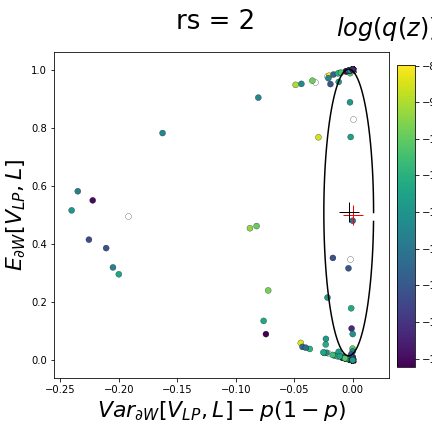
\includegraphics[scale=0.33]{figs/T_x_SC_full_c=0_p=50_rs=2.png}
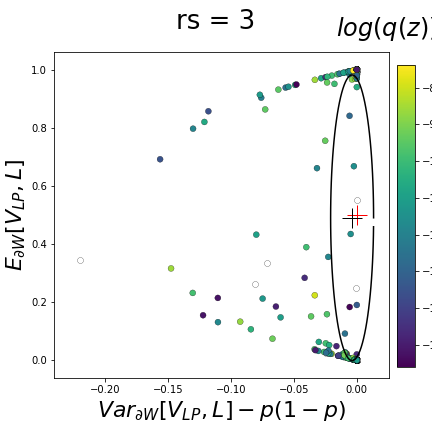
\includegraphics[scale=0.33]{figs/T_x_SC_full_c=0_p=50_rs=3.png} \\
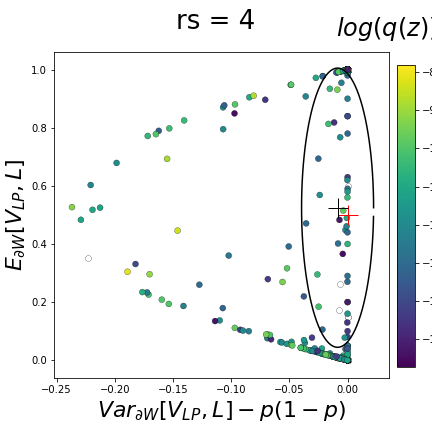
\includegraphics[scale=0.33]{figs/T_x_SC_full_c=0_p=50_rs=4.png}
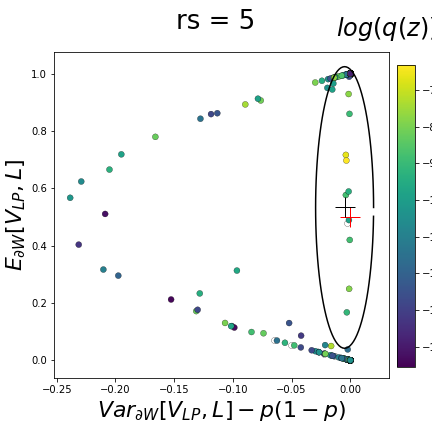
\includegraphics[scale=0.33]{figs/T_x_SC_full_c=0_p=50_rs=5.png}
\end{center}

The apparent parabola in the behavior plots is the 0-variance line of DSN samples, while the y-axis from 0-1 is the Bernoulli-variance line of DSN samples.  The network achieves the constraints by putting two modes on the extreme points of the parabola of 0-variance networks.  Ironically, this is the exact opposite of what we wanted.

In case you were wondering what happens with a $p \neq 0.5$, here is the same optimization with $p = 0.8$. Same result, except the base rates of those two expansive and decay networks are shifted from $\pi = \left[0.5, 0.5\right]$ to $\pi = \left[0.8, 0.2\right]$

EXCEPT, for random seed 4 (red), which puts all its density on the Bernoulli-variance line, NOT predominantly the 0-variance line.  At least, we know that placing all density on the Bernoulli variance in this model is learnable Maybe, that indicates that I should run the optimizations for longer, or play with new architectures.

\begin{center}
\textbf{Full model, no entropy term, p=0.8} \\
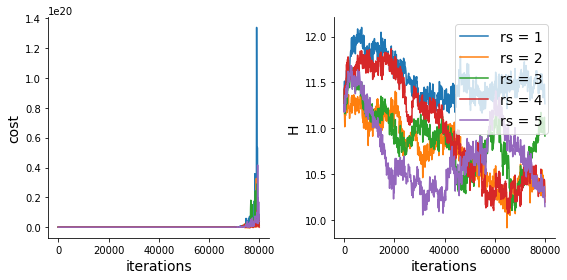
\includegraphics[scale=0.6]{figs/cost_H_SC_full_c=0_p=80.png} \\
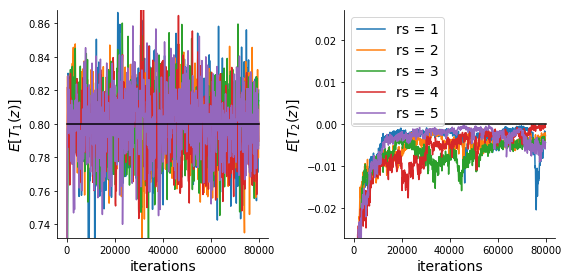
\includegraphics[scale=0.6]{figs/constraints_SC_full_c=0_p=80.png}
\end{center}
\begin{center}
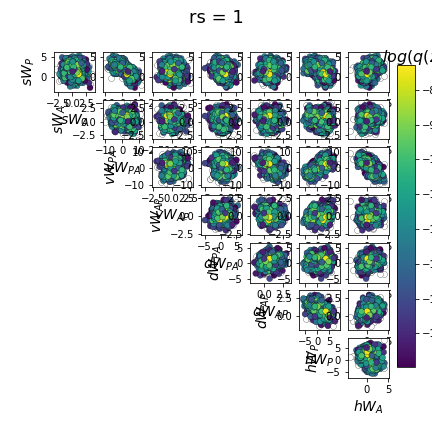
\includegraphics[scale=0.33]{figs/Z_SC_full_c=0_p=80_rs=1.png}
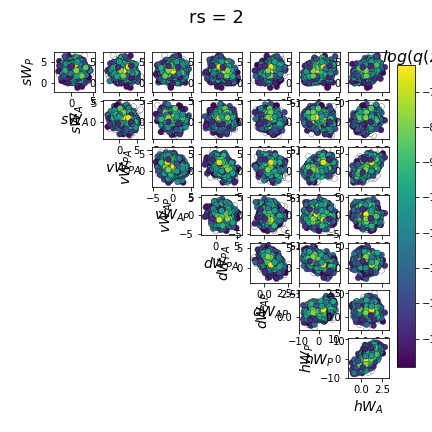
\includegraphics[scale=0.33]{figs/Z_SC_full_c=0_p=80_rs=2.png}
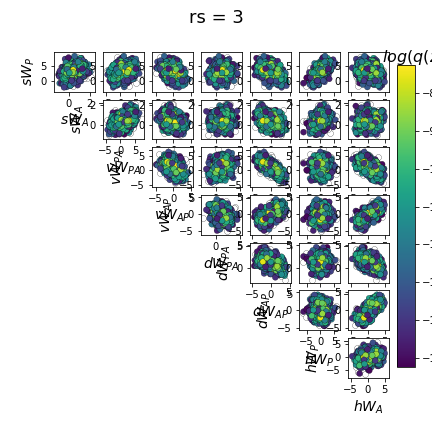
\includegraphics[scale=0.33]{figs/Z_SC_full_c=0_p=80_rs=3.png} \\
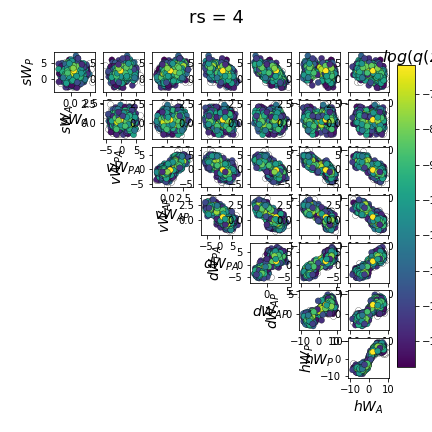
\includegraphics[scale=0.33]{figs/Z_SC_full_c=0_p=80_rs=4.png}
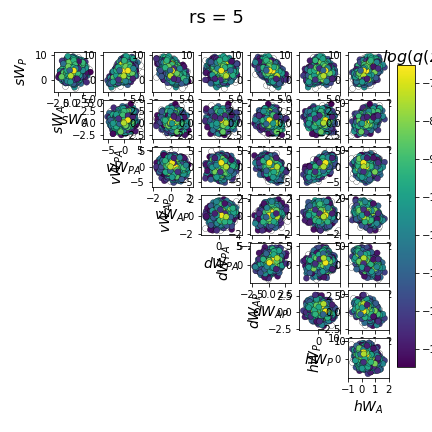
\includegraphics[scale=0.33]{figs/Z_SC_full_c=0_p=80_rs=5.png}
\end{center}
\begin{center}
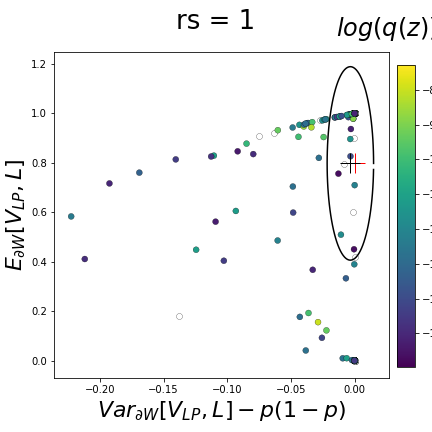
\includegraphics[scale=0.33]{figs/T_x_SC_full_c=0_p=80_rs=1.png}
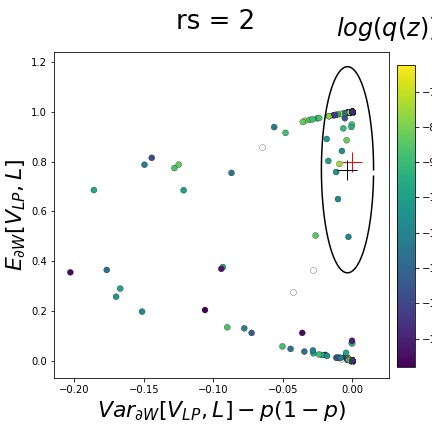
\includegraphics[scale=0.33]{figs/T_x_SC_full_c=0_p=80_rs=2.png}
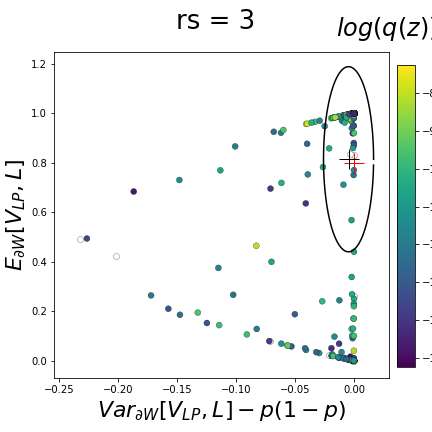
\includegraphics[scale=0.33]{figs/T_x_SC_full_c=0_p=80_rs=3.png} \\
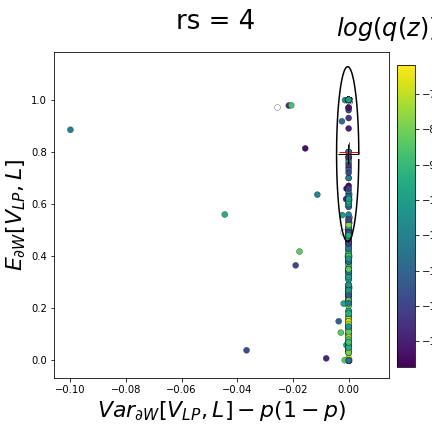
\includegraphics[scale=0.33]{figs/T_x_SC_full_c=0_p=80_rs=4.png}
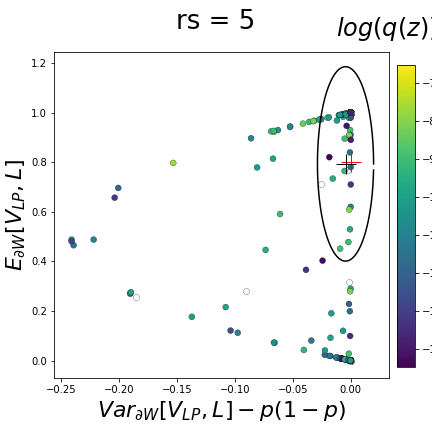
\includegraphics[scale=0.33]{figs/T_x_SC_full_c=0_p=80_rs=5.png}
\end{center}

\section{Attempt 2: Two constraints}
To combat the bimodal solutions on the extremes of the 0-variance network parabola, we can introduce a variance constraint on the estimated $\hat{p}$ of the networks.  Now, we have three constraints: 

\[E_{z \sim q_\phi} \left[ \hat{p} \right] = 0.5\]
\[E_{z \sim q\phi} \left[ Var_{\sigma \partial W} \left[ V_{LP,\text{ss}} \mid s=L, c=P, _iz \right] - \hat{p}(1 - \hat{p}) \right] = 0\]
\[Var_{z \sim q_\phi} \left[ \hat{p} \right] = 0.0001\]

\begin{center}
\textbf{Reduced model, no entropy term, $\hat{p}$ var constraint, p=0.5} \\
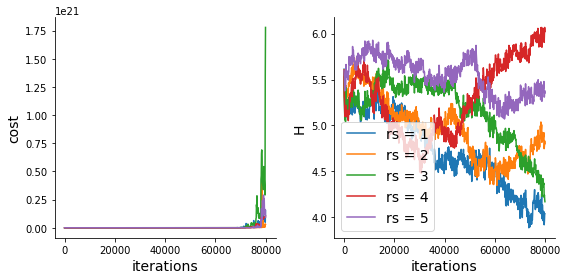
\includegraphics[scale=0.6]{figs/cost_H_SC_pvar_reduced_c=0_p=50.png} \\
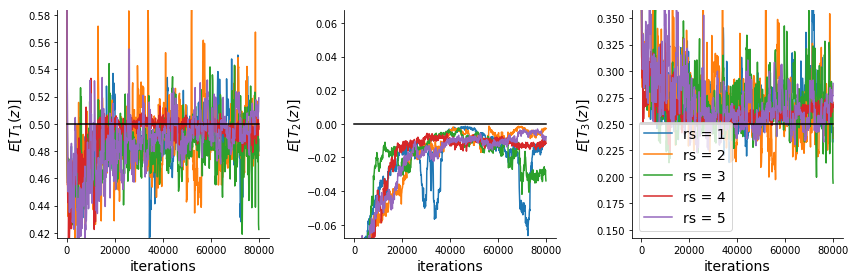
\includegraphics[scale=0.6]{figs/constraints_SC_pvar_reduced_c=0_p=50.png}
\end{center}
\begin{center}
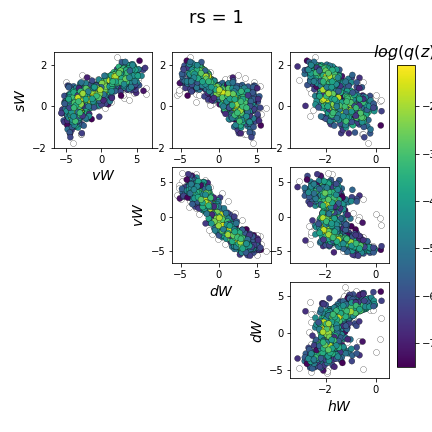
\includegraphics[scale=0.33]{figs/Z_SC_pvar_reduced_c=0_p=50_rs=1.png}
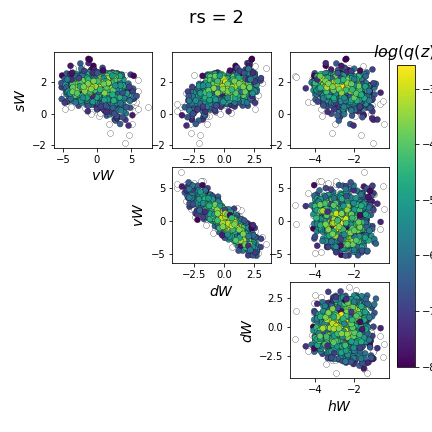
\includegraphics[scale=0.33]{figs/Z_SC_pvar_reduced_c=0_p=50_rs=2.png}
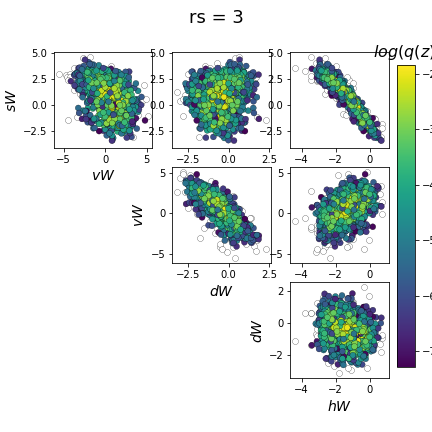
\includegraphics[scale=0.33]{figs/Z_SC_pvar_reduced_c=0_p=50_rs=3.png} \\
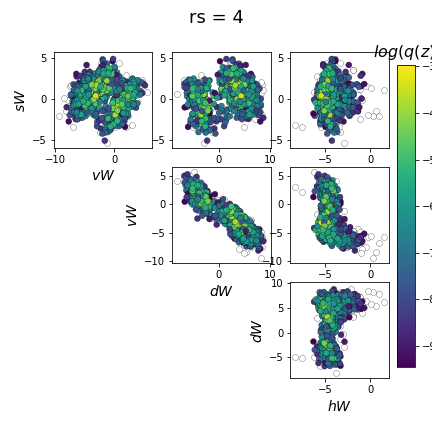
\includegraphics[scale=0.33]{figs/Z_SC_pvar_reduced_c=0_p=50_rs=4.png}
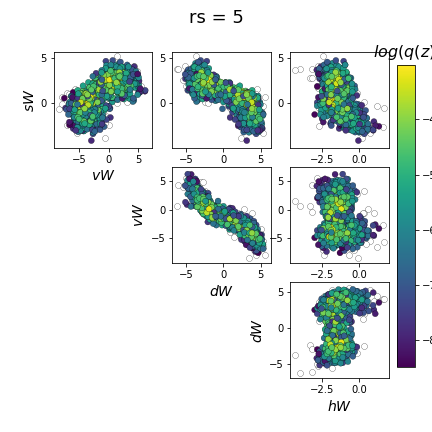
\includegraphics[scale=0.33]{figs/Z_SC_pvar_reduced_c=0_p=50_rs=5.png}
\end{center}
\begin{center}
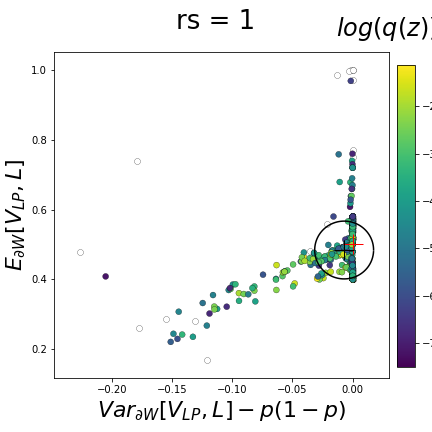
\includegraphics[scale=0.33]{figs/T_x_SC_pvar_reduced_c=0_p=50_rs=1.png}
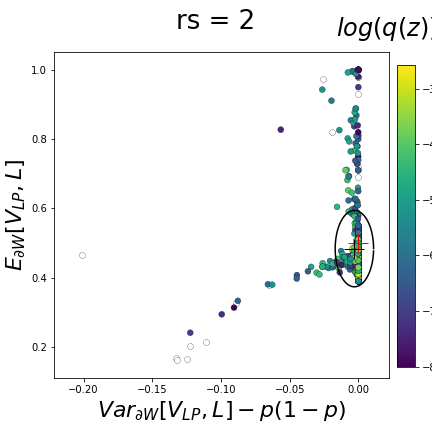
\includegraphics[scale=0.33]{figs/T_x_SC_pvar_reduced_c=0_p=50_rs=2.png}
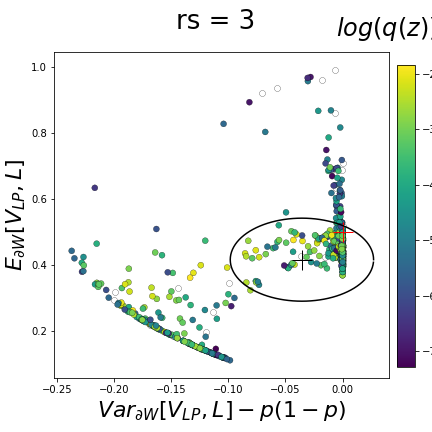
\includegraphics[scale=0.33]{figs/T_x_SC_pvar_reduced_c=0_p=50_rs=3.png} \\
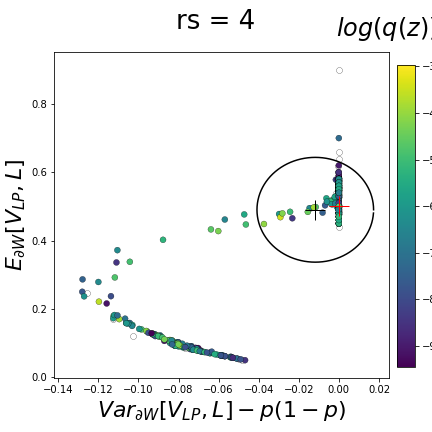
\includegraphics[scale=0.33]{figs/T_x_SC_pvar_reduced_c=0_p=50_rs=4.png}
\includegraphics[scale=0.33]{figs/T_x_SC_pvar_reduced_c=0_p=50_rs=5.png}
\end{center}

This more or less gives us the Bernoulli networks we were looking for.   But, this is only at $p = 0.5$.  What happens for other $p$, such as $p=0.8$?

\begin{center}
\textbf{Reduced model, no entropy term, $\hat{p}$ var constraint, p=0.8} \\
\includegraphics[scale=0.6]{figs/cost_H_SC_pvar_reduced_c=0_p=80.png} \\
\includegraphics[scale=0.6]{figs/constraints_SC_pvar_reduced_c=0_p=80.png}
\end{center}
\begin{center}
\includegraphics[scale=0.33]{figs/Z_SC_pvar_reduced_c=0_p=80_rs=1.png}
\includegraphics[scale=0.33]{figs/Z_SC_pvar_reduced_c=0_p=80_rs=2.png}
\includegraphics[scale=0.33]{figs/Z_SC_pvar_reduced_c=0_p=80_rs=3.png} \\
\includegraphics[scale=0.33]{figs/Z_SC_pvar_reduced_c=0_p=80_rs=4.png}
\includegraphics[scale=0.33]{figs/Z_SC_pvar_reduced_c=0_p=80_rs=5.png}
\end{center}
\begin{center}
\includegraphics[scale=0.33]{figs/T_x_SC_pvar_reduced_c=0_p=80_rs=1.png}
\includegraphics[scale=0.33]{figs/T_x_SC_pvar_reduced_c=0_p=80_rs=2.png}
\includegraphics[scale=0.33]{figs/T_x_SC_pvar_reduced_c=0_p=80_rs=3.png} \\
\includegraphics[scale=0.33]{figs/T_x_SC_pvar_reduced_c=0_p=80_rs=4.png}
\includegraphics[scale=0.33]{figs/T_x_SC_pvar_reduced_c=0_p=80_rs=5.png}
\end{center}

Without the third constraint (on the second moment of $\hat{p}$), we were able to fit the first constraint (on the first moment of $\hat{p}$) perfectly.  We hoped the third constraint would simply control the variance, but it seems that low variance in $\hat{p}$ is hard to learn.  Thus, the first and third constraints trade-off their violations optimally with respect to the cost function (the first moment undershoots, while the third moment overshoots).  As always the second moment is undershooting.

We again have a similar bimodality problem as before.  There are two main modes in the behavioral distribution ($\hat{p} = 0.5$, approx bernoulli-variance) and ($\hat{p} = 1.0$, 0-variance).   Let's try the full model, to see if an increased parameterization is able to satisfy the constraints.


\begin{center}
\textbf{Full model, no entropy term, $\hat{p}$ var constraint, p=0.8} \\
\includegraphics[scale=0.6]{figs/cost_H_SC_pvar_full_c=0_p=80.png} \\
\includegraphics[scale=0.6]{figs/constraints_SC_pvar_full_c=0_p=80.png}
\end{center}
\begin{center}
\includegraphics[scale=0.33]{figs/Z_SC_pvar_full_c=0_p=80_rs=1.png}
\includegraphics[scale=0.33]{figs/Z_SC_pvar_full_c=0_p=80_rs=2.png}
\includegraphics[scale=0.33]{figs/Z_SC_pvar_full_c=0_p=80_rs=3.png} \\
\includegraphics[scale=0.33]{figs/Z_SC_pvar_full_c=0_p=80_rs=4.png}
\includegraphics[scale=0.33]{figs/Z_SC_pvar_full_c=0_p=80_rs=5.png}
\end{center}
\begin{center}
\includegraphics[scale=0.33]{figs/T_x_SC_pvar_full_c=0_p=80_rs=1.png}
\includegraphics[scale=0.33]{figs/T_x_SC_pvar_full_c=0_p=80_rs=2.png}
\includegraphics[scale=0.33]{figs/T_x_SC_pvar_full_c=0_p=80_rs=3.png} \\
\includegraphics[scale=0.33]{figs/T_x_SC_pvar_full_c=0_p=80_rs=4.png}
\includegraphics[scale=0.33]{figs/T_x_SC_pvar_full_c=0_p=80_rs=5.png}
\end{center}

Encouragingly, most of the density of the DSN is on the Bernoulli-networks line, although we still have the too much variance due to constraint violation.

\bibliography{dsn}
\bibliographystyle{unsrt}

\end{document}

